\documentclass[]{article}
\usepackage{lmodern}
\usepackage{amssymb,amsmath}
\usepackage{ifxetex,ifluatex}
\usepackage{fixltx2e} % provides \textsubscript
\ifnum 0\ifxetex 1\fi\ifluatex 1\fi=0 % if pdftex
  \usepackage[T1]{fontenc}
  \usepackage[utf8]{inputenc}
\else % if luatex or xelatex
  \ifxetex
    \usepackage{mathspec}
  \else
    \usepackage{fontspec}
  \fi
  \defaultfontfeatures{Ligatures=TeX,Scale=MatchLowercase}
\fi
% use upquote if available, for straight quotes in verbatim environments
\IfFileExists{upquote.sty}{\usepackage{upquote}}{}
% use microtype if available
\IfFileExists{microtype.sty}{%
\usepackage{microtype}
\UseMicrotypeSet[protrusion]{basicmath} % disable protrusion for tt fonts
}{}
\usepackage[margin=1in]{geometry}
\usepackage{hyperref}
\hypersetup{unicode=true,
            pdftitle={hw5},
            pdfauthor={Kaicheng Luo},
            pdfborder={0 0 0},
            breaklinks=true}
\urlstyle{same}  % don't use monospace font for urls
\usepackage{color}
\usepackage{fancyvrb}
\newcommand{\VerbBar}{|}
\newcommand{\VERB}{\Verb[commandchars=\\\{\}]}
\DefineVerbatimEnvironment{Highlighting}{Verbatim}{commandchars=\\\{\}}
% Add ',fontsize=\small' for more characters per line
\usepackage{framed}
\definecolor{shadecolor}{RGB}{248,248,248}
\newenvironment{Shaded}{\begin{snugshade}}{\end{snugshade}}
\newcommand{\KeywordTok}[1]{\textcolor[rgb]{0.13,0.29,0.53}{\textbf{#1}}}
\newcommand{\DataTypeTok}[1]{\textcolor[rgb]{0.13,0.29,0.53}{#1}}
\newcommand{\DecValTok}[1]{\textcolor[rgb]{0.00,0.00,0.81}{#1}}
\newcommand{\BaseNTok}[1]{\textcolor[rgb]{0.00,0.00,0.81}{#1}}
\newcommand{\FloatTok}[1]{\textcolor[rgb]{0.00,0.00,0.81}{#1}}
\newcommand{\ConstantTok}[1]{\textcolor[rgb]{0.00,0.00,0.00}{#1}}
\newcommand{\CharTok}[1]{\textcolor[rgb]{0.31,0.60,0.02}{#1}}
\newcommand{\SpecialCharTok}[1]{\textcolor[rgb]{0.00,0.00,0.00}{#1}}
\newcommand{\StringTok}[1]{\textcolor[rgb]{0.31,0.60,0.02}{#1}}
\newcommand{\VerbatimStringTok}[1]{\textcolor[rgb]{0.31,0.60,0.02}{#1}}
\newcommand{\SpecialStringTok}[1]{\textcolor[rgb]{0.31,0.60,0.02}{#1}}
\newcommand{\ImportTok}[1]{#1}
\newcommand{\CommentTok}[1]{\textcolor[rgb]{0.56,0.35,0.01}{\textit{#1}}}
\newcommand{\DocumentationTok}[1]{\textcolor[rgb]{0.56,0.35,0.01}{\textbf{\textit{#1}}}}
\newcommand{\AnnotationTok}[1]{\textcolor[rgb]{0.56,0.35,0.01}{\textbf{\textit{#1}}}}
\newcommand{\CommentVarTok}[1]{\textcolor[rgb]{0.56,0.35,0.01}{\textbf{\textit{#1}}}}
\newcommand{\OtherTok}[1]{\textcolor[rgb]{0.56,0.35,0.01}{#1}}
\newcommand{\FunctionTok}[1]{\textcolor[rgb]{0.00,0.00,0.00}{#1}}
\newcommand{\VariableTok}[1]{\textcolor[rgb]{0.00,0.00,0.00}{#1}}
\newcommand{\ControlFlowTok}[1]{\textcolor[rgb]{0.13,0.29,0.53}{\textbf{#1}}}
\newcommand{\OperatorTok}[1]{\textcolor[rgb]{0.81,0.36,0.00}{\textbf{#1}}}
\newcommand{\BuiltInTok}[1]{#1}
\newcommand{\ExtensionTok}[1]{#1}
\newcommand{\PreprocessorTok}[1]{\textcolor[rgb]{0.56,0.35,0.01}{\textit{#1}}}
\newcommand{\AttributeTok}[1]{\textcolor[rgb]{0.77,0.63,0.00}{#1}}
\newcommand{\RegionMarkerTok}[1]{#1}
\newcommand{\InformationTok}[1]{\textcolor[rgb]{0.56,0.35,0.01}{\textbf{\textit{#1}}}}
\newcommand{\WarningTok}[1]{\textcolor[rgb]{0.56,0.35,0.01}{\textbf{\textit{#1}}}}
\newcommand{\AlertTok}[1]{\textcolor[rgb]{0.94,0.16,0.16}{#1}}
\newcommand{\ErrorTok}[1]{\textcolor[rgb]{0.64,0.00,0.00}{\textbf{#1}}}
\newcommand{\NormalTok}[1]{#1}
\usepackage{graphicx,grffile}
\makeatletter
\def\maxwidth{\ifdim\Gin@nat@width>\linewidth\linewidth\else\Gin@nat@width\fi}
\def\maxheight{\ifdim\Gin@nat@height>\textheight\textheight\else\Gin@nat@height\fi}
\makeatother
% Scale images if necessary, so that they will not overflow the page
% margins by default, and it is still possible to overwrite the defaults
% using explicit options in \includegraphics[width, height, ...]{}
\setkeys{Gin}{width=\maxwidth,height=\maxheight,keepaspectratio}
\IfFileExists{parskip.sty}{%
\usepackage{parskip}
}{% else
\setlength{\parindent}{0pt}
\setlength{\parskip}{6pt plus 2pt minus 1pt}
}
\setlength{\emergencystretch}{3em}  % prevent overfull lines
\providecommand{\tightlist}{%
  \setlength{\itemsep}{0pt}\setlength{\parskip}{0pt}}
\setcounter{secnumdepth}{0}
% Redefines (sub)paragraphs to behave more like sections
\ifx\paragraph\undefined\else
\let\oldparagraph\paragraph
\renewcommand{\paragraph}[1]{\oldparagraph{#1}\mbox{}}
\fi
\ifx\subparagraph\undefined\else
\let\oldsubparagraph\subparagraph
\renewcommand{\subparagraph}[1]{\oldsubparagraph{#1}\mbox{}}
\fi

%%% Use protect on footnotes to avoid problems with footnotes in titles
\let\rmarkdownfootnote\footnote%
\def\footnote{\protect\rmarkdownfootnote}

%%% Change title format to be more compact
\usepackage{titling}

% Create subtitle command for use in maketitle
\providecommand{\subtitle}[1]{
  \posttitle{
    \begin{center}\large#1\end{center}
    }
}

\setlength{\droptitle}{-2em}

  \title{hw5}
    \pretitle{\vspace{\droptitle}\centering\huge}
  \posttitle{\par}
    \author{Kaicheng Luo}
    \preauthor{\centering\large\emph}
  \postauthor{\par}
      \predate{\centering\large\emph}
  \postdate{\par}
    \date{2019/10/9}


\begin{document}
\maketitle

\begin{Shaded}
\begin{Highlighting}[]
\KeywordTok{set.seed}\NormalTok{(}\DecValTok{10000}\NormalTok{)}
\CommentTok{# Data Processing}
\NormalTok{day <-}\StringTok{ }\KeywordTok{read.csv}\NormalTok{(}\StringTok{"day.csv"}\NormalTok{)}
\NormalTok{hour <-}\StringTok{ }\KeywordTok{read.csv}\NormalTok{(}\StringTok{"hour.csv"}\NormalTok{)}
\NormalTok{data_day <-}\StringTok{ }\KeywordTok{subset}\NormalTok{(day, yr }\OperatorTok{==}\StringTok{ }\DecValTok{0}\NormalTok{)}
\NormalTok{data_day <-}\StringTok{ }\NormalTok{data_day }\OperatorTok
\StringTok{  }\KeywordTok{mutate}\NormalTok{(}\DataTypeTok{clearday =} \KeywordTok{ifelse}\NormalTok{(weathersit }\OperatorTok{==}\StringTok{ }\DecValTok{1}\NormalTok{, }\DecValTok{1}\NormalTok{, }\DecValTok{0}\NormalTok{))}
\NormalTok{data_day <-}\StringTok{ }\NormalTok{data_day }\OperatorTok
\StringTok{  }\KeywordTok{mutate}\NormalTok{(}\DataTypeTok{temp =}\NormalTok{ (temp}\OperatorTok{-}\KeywordTok{min}\NormalTok{(temp))}\OperatorTok{/}\NormalTok{(}\KeywordTok{max}\NormalTok{(temp)}\OperatorTok{-}\KeywordTok{min}\NormalTok{(temp)))}
\end{Highlighting}
\end{Shaded}

\begin{Shaded}
\begin{Highlighting}[]
\CommentTok{# Fitting Models}
\NormalTok{model_}\DecValTok{1}\NormalTok{ <-}\StringTok{ }\KeywordTok{lm}\NormalTok{(registered }\OperatorTok{~}\StringTok{ }\NormalTok{temp, }\DataTypeTok{data =}\NormalTok{ data_day)}
\NormalTok{model_}\DecValTok{2}\NormalTok{ <-}\StringTok{ }\KeywordTok{lm}\NormalTok{(registered }\OperatorTok{~}\StringTok{ }\NormalTok{temp }\OperatorTok{+}\StringTok{ }\KeywordTok{I}\NormalTok{(temp}\OperatorTok{^}\DecValTok{2}\NormalTok{), }\DataTypeTok{data =}\NormalTok{ data_day)}
\NormalTok{model_}\DecValTok{3}\NormalTok{ <-}\StringTok{ }\KeywordTok{lm}\NormalTok{(registered }\OperatorTok{~}\StringTok{ }\NormalTok{temp }\OperatorTok{+}\StringTok{ }\KeywordTok{I}\NormalTok{(temp}\OperatorTok{^}\DecValTok{2}\NormalTok{) }\OperatorTok{+}\StringTok{ }\NormalTok{workingday, }\DataTypeTok{data =}\NormalTok{ data_day)}
\NormalTok{model_}\DecValTok{4}\NormalTok{ <-}\StringTok{ }\KeywordTok{lm}\NormalTok{(registered }\OperatorTok{~}\StringTok{ }\NormalTok{temp }\OperatorTok{+}\StringTok{ }\KeywordTok{I}\NormalTok{(temp}\OperatorTok{^}\DecValTok{2}\NormalTok{) }\OperatorTok{+}\StringTok{ }\NormalTok{workingday }\OperatorTok{+}\StringTok{ }\NormalTok{clearday, }\DataTypeTok{data =}\NormalTok{ data_day)}
\NormalTok{model_}\DecValTok{5}\NormalTok{ <-}\StringTok{ }\KeywordTok{lm}\NormalTok{(registered }\OperatorTok{~}\StringTok{ }\NormalTok{temp }\OperatorTok{+}\StringTok{ }\KeywordTok{I}\NormalTok{(temp}\OperatorTok{^}\DecValTok{2}\NormalTok{) }\OperatorTok{+}\StringTok{ }\NormalTok{workingday }\OperatorTok{+}\StringTok{ }\NormalTok{clearday }\OperatorTok{+}\StringTok{ }\NormalTok{temp}\OperatorTok{*}\NormalTok{workingday, }\DataTypeTok{data =}\NormalTok{ data_day)}
\CommentTok{# stargazer(model_1, model_2, model_3, model_4, model_5, type = 'latex')}
\end{Highlighting}
\end{Shaded}

\begin{Shaded}
\begin{Highlighting}[]
\CommentTok{# Basic Model Comparison}
\NormalTok{MSE <-}\StringTok{ }\KeywordTok{rep}\NormalTok{(}\DecValTok{0}\NormalTok{,}\DecValTok{5}\NormalTok{)}
\NormalTok{MSE[}\DecValTok{1}\NormalTok{] =}\StringTok{ }\KeywordTok{mean}\NormalTok{(model_}\DecValTok{1}\OperatorTok{$}\NormalTok{residuals}\OperatorTok{^}\DecValTok{2}\NormalTok{)}
\NormalTok{MSE[}\DecValTok{2}\NormalTok{] =}\StringTok{ }\KeywordTok{mean}\NormalTok{(model_}\DecValTok{2}\OperatorTok{$}\NormalTok{residuals}\OperatorTok{^}\DecValTok{2}\NormalTok{)}
\NormalTok{MSE[}\DecValTok{3}\NormalTok{] =}\StringTok{ }\KeywordTok{mean}\NormalTok{(model_}\DecValTok{3}\OperatorTok{$}\NormalTok{residuals}\OperatorTok{^}\DecValTok{2}\NormalTok{)}
\NormalTok{MSE[}\DecValTok{4}\NormalTok{] =}\StringTok{ }\KeywordTok{mean}\NormalTok{(model_}\DecValTok{4}\OperatorTok{$}\NormalTok{residuals}\OperatorTok{^}\DecValTok{2}\NormalTok{)}
\NormalTok{MSE[}\DecValTok{5}\NormalTok{] =}\StringTok{ }\KeywordTok{mean}\NormalTok{(model_}\DecValTok{5}\OperatorTok{$}\NormalTok{residuals}\OperatorTok{^}\DecValTok{2}\NormalTok{)}
\NormalTok{MSE }\OperatorTok\StringTok{ }\KeywordTok{data.frame}\NormalTok{(}\StringTok{"Complexity"}\NormalTok{ =}\StringTok{ }\DecValTok{1}\OperatorTok{:}\DecValTok{5}\NormalTok{, }\DataTypeTok{MSE =}\NormalTok{ MSE) }\OperatorTok
\StringTok{  }\KeywordTok{ggplot}\NormalTok{() }\OperatorTok{+}\StringTok{ }\KeywordTok{theme_bw}\NormalTok{() }\OperatorTok{+}
\StringTok{  }\KeywordTok{geom_line}\NormalTok{(}\KeywordTok{aes}\NormalTok{(}\DataTypeTok{x =}\NormalTok{ Complexity, }\DataTypeTok{y =}\NormalTok{ MSE), }\DataTypeTok{color =} \StringTok{'maroon'}\NormalTok{, }\DataTypeTok{size =} \DecValTok{1}\NormalTok{) }\OperatorTok{+}
\StringTok{  }\KeywordTok{labs}\NormalTok{(}
    \DataTypeTok{title =} \StringTok{"MSE of the Bike Sharing Model w.r.t # of Regressors"}\NormalTok{,}
    \DataTypeTok{caption =} \StringTok{"Dataset: 2011 Washington Bike Sharing Data (Hadi Fanaee)"}
\NormalTok{  )}
\end{Highlighting}
\end{Shaded}

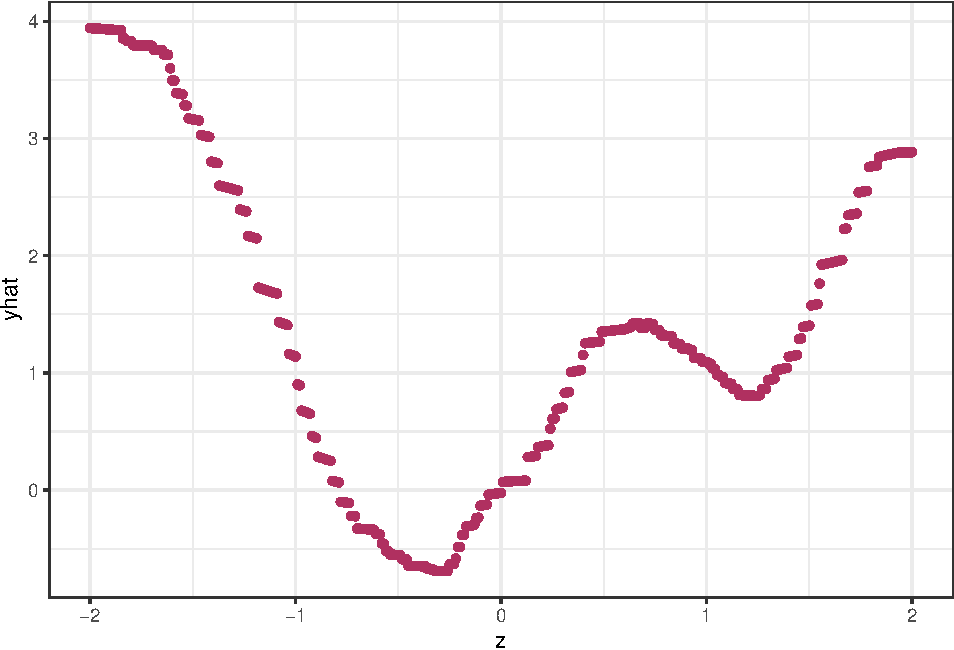
\includegraphics{hw5_files/figure-latex/unnamed-chunk-3-1.pdf}

\begin{Shaded}
\begin{Highlighting}[]
\CommentTok{# Hold-out Method}
\NormalTok{subs <-}\StringTok{ }\KeywordTok{sample}\NormalTok{(}\DecValTok{365}\NormalTok{, }\DecValTok{292}\NormalTok{)}
\CommentTok{# Subtracting Training and Test Set}
\NormalTok{trainingSet <-}\StringTok{ }\NormalTok{data_day[subs, ]}
\NormalTok{testSet <-}\StringTok{ }\NormalTok{data_day[}\OperatorTok{-}\NormalTok{subs, ]}
\CommentTok{# Train the Model}
\NormalTok{model_}\DecValTok{1}\NormalTok{ <-}\StringTok{ }\KeywordTok{lm}\NormalTok{(registered }\OperatorTok{~}\StringTok{ }\NormalTok{temp, }\DataTypeTok{data =}\NormalTok{ trainingSet)}
\NormalTok{model_}\DecValTok{2}\NormalTok{ <-}\StringTok{ }\KeywordTok{lm}\NormalTok{(registered }\OperatorTok{~}\StringTok{ }\NormalTok{temp }\OperatorTok{+}\StringTok{ }\KeywordTok{I}\NormalTok{(temp}\OperatorTok{^}\DecValTok{2}\NormalTok{), }\DataTypeTok{data =}\NormalTok{ trainingSet)}
\NormalTok{model_}\DecValTok{3}\NormalTok{ <-}\StringTok{ }\KeywordTok{lm}\NormalTok{(registered }\OperatorTok{~}\StringTok{ }\NormalTok{temp }\OperatorTok{+}\StringTok{ }\KeywordTok{I}\NormalTok{(temp}\OperatorTok{^}\DecValTok{2}\NormalTok{) }\OperatorTok{+}\StringTok{ }\NormalTok{workingday, }\DataTypeTok{data =}\NormalTok{ trainingSet)}
\NormalTok{model_}\DecValTok{4}\NormalTok{ <-}\StringTok{ }\KeywordTok{lm}\NormalTok{(registered }\OperatorTok{~}\StringTok{ }\NormalTok{temp }\OperatorTok{+}\StringTok{ }\KeywordTok{I}\NormalTok{(temp}\OperatorTok{^}\DecValTok{2}\NormalTok{) }\OperatorTok{+}\StringTok{ }\NormalTok{workingday }\OperatorTok{+}\StringTok{ }\NormalTok{clearday, }\DataTypeTok{data =}\NormalTok{ trainingSet)}
\NormalTok{model_}\DecValTok{5}\NormalTok{ <-}\StringTok{ }\KeywordTok{lm}\NormalTok{(registered }\OperatorTok{~}\StringTok{ }\NormalTok{temp }\OperatorTok{+}\StringTok{ }\KeywordTok{I}\NormalTok{(temp}\OperatorTok{^}\DecValTok{2}\NormalTok{) }\OperatorTok{+}\StringTok{ }\NormalTok{workingday }\OperatorTok{+}\StringTok{ }\NormalTok{clearday }\OperatorTok{+}\StringTok{ }\NormalTok{temp}\OperatorTok{*}\NormalTok{workingday, }\DataTypeTok{data =}\NormalTok{ trainingSet)}
\CommentTok{# Compute the training MSE}
\NormalTok{MSE <-}\StringTok{ }\KeywordTok{rep}\NormalTok{(}\DecValTok{0}\NormalTok{,}\DecValTok{5}\NormalTok{)}
\NormalTok{MSE[}\DecValTok{1}\NormalTok{] =}\StringTok{ }\KeywordTok{mean}\NormalTok{(model_}\DecValTok{1}\OperatorTok{$}\NormalTok{residuals}\OperatorTok{^}\DecValTok{2}\NormalTok{)}
\NormalTok{MSE[}\DecValTok{2}\NormalTok{] =}\StringTok{ }\KeywordTok{mean}\NormalTok{(model_}\DecValTok{2}\OperatorTok{$}\NormalTok{residuals}\OperatorTok{^}\DecValTok{2}\NormalTok{)}
\NormalTok{MSE[}\DecValTok{3}\NormalTok{] =}\StringTok{ }\KeywordTok{mean}\NormalTok{(model_}\DecValTok{3}\OperatorTok{$}\NormalTok{residuals}\OperatorTok{^}\DecValTok{2}\NormalTok{)}
\NormalTok{MSE[}\DecValTok{4}\NormalTok{] =}\StringTok{ }\KeywordTok{mean}\NormalTok{(model_}\DecValTok{4}\OperatorTok{$}\NormalTok{residuals}\OperatorTok{^}\DecValTok{2}\NormalTok{)}
\NormalTok{MSE[}\DecValTok{5}\NormalTok{] =}\StringTok{ }\KeywordTok{mean}\NormalTok{(model_}\DecValTok{5}\OperatorTok{$}\NormalTok{residuals}\OperatorTok{^}\DecValTok{2}\NormalTok{)}
\CommentTok{# Compute the test MSE}
\NormalTok{test_MSE =}\StringTok{ }\KeywordTok{rep}\NormalTok{(}\DecValTok{0}\NormalTok{,}\DecValTok{5}\NormalTok{)}
\NormalTok{testX =}\StringTok{ }\KeywordTok{cbind}\NormalTok{(}\DecValTok{1}\NormalTok{, testSet}\OperatorTok{$}\NormalTok{temp)}
\NormalTok{test_MSE[}\DecValTok{1}\NormalTok{] =}\StringTok{ }\KeywordTok{mean}\NormalTok{((testSet[, }\StringTok{"registered"}\NormalTok{] }\OperatorTok{-}\StringTok{ }\NormalTok{testX }\OperatorTok\StringTok{ }\NormalTok{model_}\DecValTok{1}\OperatorTok{$}\NormalTok{coefficients)}\OperatorTok{^}\DecValTok{2}\NormalTok{)}
\NormalTok{testX =}\StringTok{ }\KeywordTok{cbind}\NormalTok{(}\DecValTok{1}\NormalTok{, testSet}\OperatorTok{$}\NormalTok{temp, testSet}\OperatorTok{$}\NormalTok{temp}\OperatorTok{^}\DecValTok{2}\NormalTok{)}
\NormalTok{test_MSE[}\DecValTok{2}\NormalTok{] =}\StringTok{ }\KeywordTok{mean}\NormalTok{((testSet[, }\StringTok{"registered"}\NormalTok{] }\OperatorTok{-}\StringTok{ }\NormalTok{testX }\OperatorTok\StringTok{ }\NormalTok{model_}\DecValTok{2}\OperatorTok{$}\NormalTok{coefficients)}\OperatorTok{^}\DecValTok{2}\NormalTok{)}
\NormalTok{testX =}\StringTok{ }\KeywordTok{cbind}\NormalTok{(}\DecValTok{1}\NormalTok{, testSet}\OperatorTok{$}\NormalTok{temp, testSet}\OperatorTok{$}\NormalTok{temp}\OperatorTok{^}\DecValTok{2}\NormalTok{, testSet}\OperatorTok{$}\NormalTok{workingday)}
\NormalTok{test_MSE[}\DecValTok{3}\NormalTok{] =}\StringTok{ }\KeywordTok{mean}\NormalTok{((testSet[, }\StringTok{"registered"}\NormalTok{] }\OperatorTok{-}\StringTok{ }\NormalTok{testX }\OperatorTok\StringTok{ }\NormalTok{model_}\DecValTok{3}\OperatorTok{$}\NormalTok{coefficients)}\OperatorTok{^}\DecValTok{2}\NormalTok{)}
\NormalTok{testX =}\StringTok{ }\KeywordTok{cbind}\NormalTok{(}\DecValTok{1}\NormalTok{, testSet}\OperatorTok{$}\NormalTok{temp, testSet}\OperatorTok{$}\NormalTok{temp}\OperatorTok{^}\DecValTok{2}\NormalTok{, testSet}\OperatorTok{$}\NormalTok{workingday, testSet}\OperatorTok{$}\NormalTok{clearday)}
\NormalTok{test_MSE[}\DecValTok{4}\NormalTok{] =}\StringTok{ }\KeywordTok{mean}\NormalTok{((testSet[, }\StringTok{"registered"}\NormalTok{] }\OperatorTok{-}\StringTok{ }\NormalTok{testX }\OperatorTok\StringTok{ }\NormalTok{model_}\DecValTok{4}\OperatorTok{$}\NormalTok{coefficients)}\OperatorTok{^}\DecValTok{2}\NormalTok{)}
\NormalTok{testX =}\StringTok{ }\KeywordTok{cbind}\NormalTok{(}\DecValTok{1}\NormalTok{, testSet}\OperatorTok{$}\NormalTok{temp, testSet}\OperatorTok{$}\NormalTok{temp}\OperatorTok{^}\DecValTok{2}\NormalTok{, testSet}\OperatorTok{$}\NormalTok{workingday, testSet}\OperatorTok{$}\NormalTok{clearday, testSet}\OperatorTok{$}\NormalTok{temp }\OperatorTok{*}\StringTok{ }\NormalTok{testSet}\OperatorTok{$}\NormalTok{workingday)}
\NormalTok{test_MSE[}\DecValTok{5}\NormalTok{] =}\StringTok{ }\KeywordTok{mean}\NormalTok{((testSet[, }\StringTok{"registered"}\NormalTok{] }\OperatorTok{-}\StringTok{ }\NormalTok{testX }\OperatorTok\StringTok{ }\NormalTok{model_}\DecValTok{5}\OperatorTok{$}\NormalTok{coefficients)}\OperatorTok{^}\DecValTok{2}\NormalTok{)}
\end{Highlighting}
\end{Shaded}

\begin{Shaded}
\begin{Highlighting}[]
\KeywordTok{data.frame}\NormalTok{(}\StringTok{"Complexity"}\NormalTok{ =}\StringTok{ }\DecValTok{1}\OperatorTok{:}\DecValTok{5}\NormalTok{, }\DataTypeTok{training_MSE =}\NormalTok{ MSE, }\DataTypeTok{test_MSE =}\NormalTok{ test_MSE) }\OperatorTok
\StringTok{  }\KeywordTok{ggplot}\NormalTok{() }\OperatorTok{+}\StringTok{ }\KeywordTok{theme_bw}\NormalTok{() }\OperatorTok{+}
\StringTok{  }\KeywordTok{geom_line}\NormalTok{(}\KeywordTok{aes}\NormalTok{(}\DataTypeTok{x =}\NormalTok{ Complexity, }\DataTypeTok{y =}\NormalTok{ training_MSE), }\DataTypeTok{color =} \StringTok{'maroon'}\NormalTok{, }\DataTypeTok{size =} \DecValTok{1}\NormalTok{) }\OperatorTok{+}
\StringTok{  }\KeywordTok{geom_line}\NormalTok{(}\KeywordTok{aes}\NormalTok{(}\DataTypeTok{x =}\NormalTok{ Complexity, }\DataTypeTok{y =}\NormalTok{ test_MSE), }\DataTypeTok{color =} \StringTok{'purple'}\NormalTok{, }\DataTypeTok{size =} \DecValTok{1}\NormalTok{) }\OperatorTok{+}
\StringTok{  }\KeywordTok{labs}\NormalTok{(}
    \DataTypeTok{title =} \StringTok{"MSE of the Bike Sharing Model w.r.t # of Regressors"}\NormalTok{,}
    \DataTypeTok{caption =} \StringTok{"Dataset: 2011 Washington Bike Sharing Data (Hadi Fanaee)"}
\NormalTok{  )}
\end{Highlighting}
\end{Shaded}

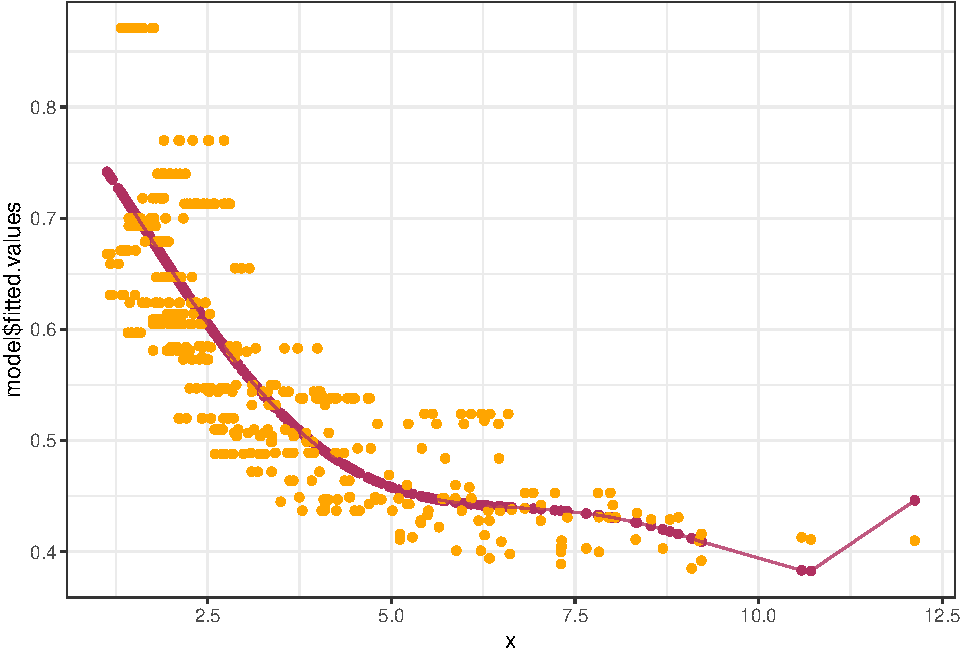
\includegraphics{hw5_files/figure-latex/unnamed-chunk-5-1.pdf}

\section*{Problem 5 Bike Sharing: Cross-validation}

\begin{Shaded}
\begin{Highlighting}[]
\CommentTok{# Create 10 folds}
\NormalTok{fold <-}\StringTok{ }\KeywordTok{list}\NormalTok{()}
\NormalTok{tempdata <-}\StringTok{ }\NormalTok{data_day}
\NormalTok{i =}\StringTok{ }\DecValTok{1}
\NormalTok{data_day <-}\StringTok{ }\NormalTok{data_day }\OperatorTok
\StringTok{  }\KeywordTok{mutate}\NormalTok{(}\DataTypeTok{fold =} \DecValTok{0}\NormalTok{)}
\ControlFlowTok{while}\NormalTok{ (}\KeywordTok{nrow}\NormalTok{(tempdata)}\OperatorTok{>}\DecValTok{5}\NormalTok{)\{}
\NormalTok{  fold[[i]] <-}\StringTok{   }\KeywordTok{sample_n}\NormalTok{(tempdata, }\DecValTok{36}\NormalTok{)}
\NormalTok{  tempdata <-}\StringTok{ }\NormalTok{tempdata }\OperatorTok
\StringTok{    }\KeywordTok{filter}\NormalTok{(}\OperatorTok{!}\NormalTok{(instant }\OperatorTok\StringTok{ }\NormalTok{fold[[i]]}\OperatorTok{$}\NormalTok{instant))}
\NormalTok{  i =}\StringTok{ }\NormalTok{i}\OperatorTok{+}\DecValTok{1}
\NormalTok{\}}
\ControlFlowTok{for}\NormalTok{ (i }\ControlFlowTok{in} \DecValTok{1}\OperatorTok{:}\KeywordTok{nrow}\NormalTok{(data_day))\{}
  \ControlFlowTok{for}\NormalTok{ (j }\ControlFlowTok{in} \DecValTok{1}\OperatorTok{:}\DecValTok{10}\NormalTok{)\{}
    \ControlFlowTok{if}\NormalTok{ (data_day}\OperatorTok{$}\NormalTok{instant[i] }\OperatorTok\StringTok{ }\NormalTok{fold[[j]]}\OperatorTok{$}\NormalTok{instant)\{}
\NormalTok{      data_day}\OperatorTok{$}\NormalTok{fold[i] =}\StringTok{ }\NormalTok{j}
\NormalTok{    \}}
\NormalTok{  \}}
\NormalTok{\}}
\end{Highlighting}
\end{Shaded}

\begin{Shaded}
\begin{Highlighting}[]
\NormalTok{MSE <-}\StringTok{ }\KeywordTok{matrix}\NormalTok{(}\DecValTok{0}\NormalTok{, }\DataTypeTok{nrow =} \DecValTok{5}\NormalTok{, }\DataTypeTok{ncol =} \DecValTok{10}\NormalTok{)}
\ControlFlowTok{for}\NormalTok{ (i }\ControlFlowTok{in} \DecValTok{1}\OperatorTok{:}\DecValTok{10}\NormalTok{)\{}
\NormalTok{  trainingSet =}\StringTok{ }\NormalTok{data_day }\OperatorTok\StringTok{ }\KeywordTok{filter}\NormalTok{(fold }\OperatorTok{!=}\StringTok{ }\NormalTok{i)}
\NormalTok{  testSet =}\StringTok{ }\NormalTok{data_day }\OperatorTok\StringTok{ }\KeywordTok{filter}\NormalTok{(fold }\OperatorTok{==}\StringTok{ }\NormalTok{i)}
\NormalTok{  model_}\DecValTok{1}\NormalTok{ <-}\StringTok{ }\KeywordTok{lm}\NormalTok{(registered }\OperatorTok{~}\StringTok{ }\NormalTok{temp, }\DataTypeTok{data =}\NormalTok{ trainingSet)}
\NormalTok{  model_}\DecValTok{2}\NormalTok{ <-}\StringTok{ }\KeywordTok{lm}\NormalTok{(registered }\OperatorTok{~}\StringTok{ }\NormalTok{temp }\OperatorTok{+}\StringTok{ }\KeywordTok{I}\NormalTok{(temp}\OperatorTok{^}\DecValTok{2}\NormalTok{), }\DataTypeTok{data =}\NormalTok{ trainingSet)}
\NormalTok{  model_}\DecValTok{3}\NormalTok{ <-}\StringTok{ }\KeywordTok{lm}\NormalTok{(registered }\OperatorTok{~}\StringTok{ }\NormalTok{temp }\OperatorTok{+}\StringTok{ }\KeywordTok{I}\NormalTok{(temp}\OperatorTok{^}\DecValTok{2}\NormalTok{) }\OperatorTok{+}\StringTok{ }\NormalTok{workingday, }\DataTypeTok{data =}\NormalTok{ trainingSet)}
\NormalTok{  model_}\DecValTok{4}\NormalTok{ <-}\StringTok{ }\KeywordTok{lm}\NormalTok{(registered }\OperatorTok{~}\StringTok{ }\NormalTok{temp }\OperatorTok{+}\StringTok{ }\KeywordTok{I}\NormalTok{(temp}\OperatorTok{^}\DecValTok{2}\NormalTok{) }\OperatorTok{+}\StringTok{ }\NormalTok{workingday }\OperatorTok{+}\StringTok{ }\NormalTok{clearday, }\DataTypeTok{data =}\NormalTok{ trainingSet)}
\NormalTok{  model_}\DecValTok{5}\NormalTok{ <-}\StringTok{ }\KeywordTok{lm}\NormalTok{(registered }\OperatorTok{~}\StringTok{ }\NormalTok{temp }\OperatorTok{+}\StringTok{ }\KeywordTok{I}\NormalTok{(temp}\OperatorTok{^}\DecValTok{2}\NormalTok{) }\OperatorTok{+}\StringTok{ }\NormalTok{workingday }\OperatorTok{+}\StringTok{ }\NormalTok{clearday }\OperatorTok{+}\StringTok{ }\NormalTok{temp}\OperatorTok{*}\NormalTok{workingday, }\DataTypeTok{data =}\NormalTok{ trainingSet)}
\NormalTok{  testX =}\StringTok{ }\KeywordTok{cbind}\NormalTok{(}\DecValTok{1}\NormalTok{, testSet}\OperatorTok{$}\NormalTok{temp)}
\NormalTok{  MSE[}\DecValTok{1}\NormalTok{, i] =}\StringTok{ }\KeywordTok{mean}\NormalTok{((testSet[, }\StringTok{"registered"}\NormalTok{] }\OperatorTok{-}\StringTok{ }\NormalTok{testX }\OperatorTok\StringTok{ }\NormalTok{model_}\DecValTok{1}\OperatorTok{$}\NormalTok{coefficients)}\OperatorTok{^}\DecValTok{2}\NormalTok{)}
\NormalTok{  testX =}\StringTok{ }\KeywordTok{cbind}\NormalTok{(}\DecValTok{1}\NormalTok{, testSet}\OperatorTok{$}\NormalTok{temp, testSet}\OperatorTok{$}\NormalTok{temp}\OperatorTok{^}\DecValTok{2}\NormalTok{)}
\NormalTok{  MSE[}\DecValTok{2}\NormalTok{, i] =}\StringTok{ }\KeywordTok{mean}\NormalTok{((testSet[, }\StringTok{"registered"}\NormalTok{] }\OperatorTok{-}\StringTok{ }\NormalTok{testX }\OperatorTok\StringTok{ }\NormalTok{model_}\DecValTok{2}\OperatorTok{$}\NormalTok{coefficients)}\OperatorTok{^}\DecValTok{2}\NormalTok{)}
\NormalTok{  testX =}\StringTok{ }\KeywordTok{cbind}\NormalTok{(}\DecValTok{1}\NormalTok{, testSet}\OperatorTok{$}\NormalTok{temp, testSet}\OperatorTok{$}\NormalTok{temp}\OperatorTok{^}\DecValTok{2}\NormalTok{, testSet}\OperatorTok{$}\NormalTok{workingday)}
\NormalTok{  MSE[}\DecValTok{3}\NormalTok{, i] =}\StringTok{ }\KeywordTok{mean}\NormalTok{((testSet[, }\StringTok{"registered"}\NormalTok{] }\OperatorTok{-}\StringTok{ }\NormalTok{testX }\OperatorTok\StringTok{ }\NormalTok{model_}\DecValTok{3}\OperatorTok{$}\NormalTok{coefficients)}\OperatorTok{^}\DecValTok{2}\NormalTok{)}
\NormalTok{  testX =}\StringTok{ }\KeywordTok{cbind}\NormalTok{(}\DecValTok{1}\NormalTok{, testSet}\OperatorTok{$}\NormalTok{temp, testSet}\OperatorTok{$}\NormalTok{temp}\OperatorTok{^}\DecValTok{2}\NormalTok{, testSet}\OperatorTok{$}\NormalTok{workingday, testSet}\OperatorTok{$}\NormalTok{clearday)}
\NormalTok{  MSE[}\DecValTok{4}\NormalTok{, i] =}\StringTok{ }\KeywordTok{mean}\NormalTok{((testSet[, }\StringTok{"registered"}\NormalTok{] }\OperatorTok{-}\StringTok{ }\NormalTok{testX }\OperatorTok\StringTok{ }\NormalTok{model_}\DecValTok{4}\OperatorTok{$}\NormalTok{coefficients)}\OperatorTok{^}\DecValTok{2}\NormalTok{)}
\NormalTok{  testX =}\StringTok{ }\KeywordTok{cbind}\NormalTok{(}\DecValTok{1}\NormalTok{, testSet}\OperatorTok{$}\NormalTok{temp, testSet}\OperatorTok{$}\NormalTok{temp}\OperatorTok{^}\DecValTok{2}\NormalTok{, testSet}\OperatorTok{$}\NormalTok{workingday, testSet}\OperatorTok{$}\NormalTok{clearday, testSet}\OperatorTok{$}\NormalTok{temp }\OperatorTok{*}\StringTok{ }\NormalTok{testSet}\OperatorTok{$}\NormalTok{workingday)}
\NormalTok{  MSE[}\DecValTok{5}\NormalTok{, i] =}\StringTok{ }\KeywordTok{mean}\NormalTok{((testSet[, }\StringTok{"registered"}\NormalTok{] }\OperatorTok{-}\StringTok{ }\NormalTok{testX }\OperatorTok\StringTok{ }\NormalTok{model_}\DecValTok{5}\OperatorTok{$}\NormalTok{coefficients)}\OperatorTok{^}\DecValTok{2}\NormalTok{)}
\NormalTok{\}}
\NormalTok{MSE}
\end{Highlighting}
\end{Shaded}

\begin{verbatim}
##          [,1]     [,2]     [,3]     [,4]     [,5]     [,6]     [,7]
## [1,] 758856.4 466304.8 509418.4 707323.6 677892.4 485899.7 521152.0
## [2,] 717297.5 469081.1 470483.5 638717.2 589642.4 438569.0 453312.3
## [3,] 648848.3 412820.9 305583.0 551156.8 436616.1 534552.3 349198.8
## [4,] 577146.7 359617.3 344021.8 391933.1 419637.6 460725.7 330256.5
## [5,] 555948.2 377214.5 344582.6 375084.5 409372.8 444682.4 349162.2
##          [,8]     [,9]    [,10]
## [1,] 443595.7 507893.4 758339.8
## [2,] 434179.4 461025.4 757344.9
## [3,] 314773.5 361993.6 648256.4
## [4,] 276733.8 342148.6 507739.0
## [5,] 277027.0 342049.1 512121.6
\end{verbatim}

\begin{Shaded}
\begin{Highlighting}[]
\NormalTok{MSE_bar <-}\StringTok{ }\KeywordTok{c}\NormalTok{()}
\ControlFlowTok{for}\NormalTok{ (i }\ControlFlowTok{in} \DecValTok{1}\OperatorTok{:}\DecValTok{5}\NormalTok{)\{}
  \KeywordTok{print}\NormalTok{(}\KeywordTok{mean}\NormalTok{(MSE[i, ]))}
\NormalTok{  MSE_bar <-}\StringTok{ }\KeywordTok{c}\NormalTok{(MSE_bar, }\KeywordTok{mean}\NormalTok{(MSE[i, ]))}
\NormalTok{\}}
\end{Highlighting}
\end{Shaded}

\begin{verbatim}
## [1] 583667.6
## [1] 542965.3
## [1] 456380
## [1] 400996
## [1] 398724.5
\end{verbatim}

\begin{Shaded}
\begin{Highlighting}[]
\KeywordTok{data.frame}\NormalTok{(}\StringTok{"Complexity"}\NormalTok{ =}\StringTok{ }\DecValTok{1}\OperatorTok{:}\DecValTok{5}\NormalTok{, }\StringTok{"kfold_MSE"}\NormalTok{ =}\StringTok{ }\NormalTok{MSE_bar) }\OperatorTok
\StringTok{  }\KeywordTok{ggplot}\NormalTok{() }\OperatorTok{+}\StringTok{ }\KeywordTok{theme_bw}\NormalTok{() }\OperatorTok{+}
\StringTok{  }\KeywordTok{geom_line}\NormalTok{(}\KeywordTok{aes}\NormalTok{(}\DataTypeTok{x =}\NormalTok{ Complexity, }\DataTypeTok{y =}\NormalTok{ kfold_MSE), }\DataTypeTok{color =} \StringTok{'maroon'}\NormalTok{, }\DataTypeTok{size =} \DecValTok{1}\NormalTok{) }\OperatorTok{+}
\StringTok{  }\KeywordTok{labs}\NormalTok{(}
    \DataTypeTok{title =} \StringTok{"MSE of the Bike Sharing Model w.r.t # of Regressors"}\NormalTok{,}
    \DataTypeTok{caption =} \StringTok{"Dataset: 2011 Washington Bike Sharing Data (Hadi Fanaee)"}
\NormalTok{  )}
\end{Highlighting}
\end{Shaded}

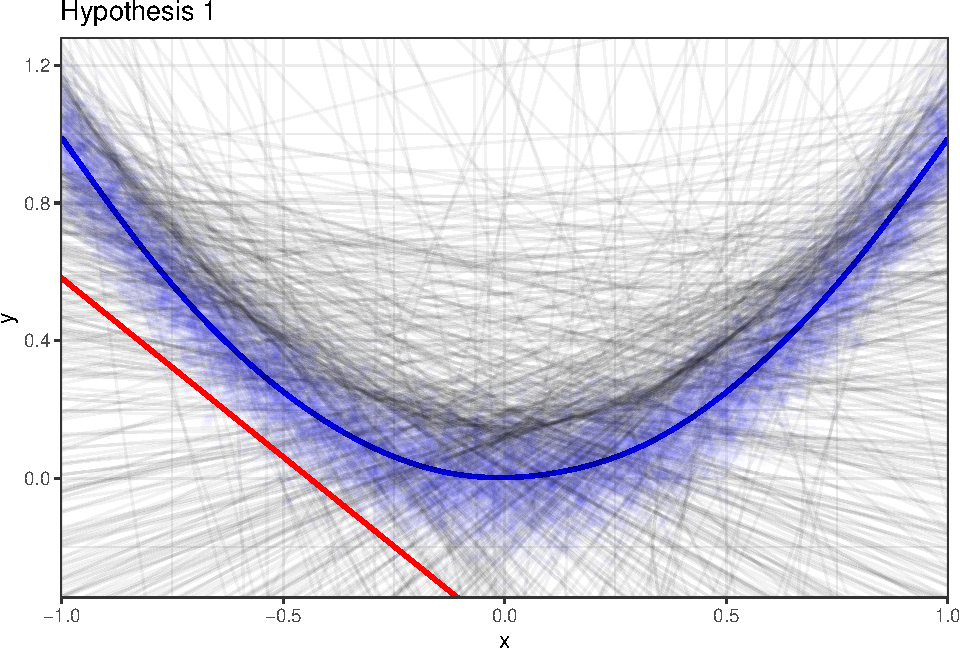
\includegraphics{hw5_files/figure-latex/unnamed-chunk-8-1.pdf}

\section*{Problem 6 BootStrap MSE}

\begin{Shaded}
\begin{Highlighting}[]
\NormalTok{MSE <-}\StringTok{ }\KeywordTok{matrix}\NormalTok{(}\DecValTok{0}\NormalTok{, }\DataTypeTok{nrow =} \DecValTok{5}\NormalTok{, }\DataTypeTok{ncol =} \DecValTok{200}\NormalTok{)}
\ControlFlowTok{for}\NormalTok{ (i }\ControlFlowTok{in} \DecValTok{1}\OperatorTok{:}\DecValTok{200}\NormalTok{)\{}
\NormalTok{  trainingSet <-}\StringTok{ }\NormalTok{data_day[}\KeywordTok{sample}\NormalTok{(}\DecValTok{365}\NormalTok{, }\DecValTok{200}\NormalTok{, }\DataTypeTok{replace =} \OtherTok{TRUE}\NormalTok{), ]}
\NormalTok{  testSet <-}\StringTok{ }\NormalTok{data_day }\OperatorTok
\StringTok{    }\KeywordTok{filter}\NormalTok{(}\OperatorTok{!}\StringTok{ }\NormalTok{instant }\OperatorTok\StringTok{ }\NormalTok{trainingSet}\OperatorTok{$}\NormalTok{instant)}
\NormalTok{  model_}\DecValTok{1}\NormalTok{ <-}\StringTok{ }\KeywordTok{lm}\NormalTok{(registered }\OperatorTok{~}\StringTok{ }\NormalTok{temp, }\DataTypeTok{data =}\NormalTok{ trainingSet)}
\NormalTok{  model_}\DecValTok{2}\NormalTok{ <-}\StringTok{ }\KeywordTok{lm}\NormalTok{(registered }\OperatorTok{~}\StringTok{ }\NormalTok{temp }\OperatorTok{+}\StringTok{ }\KeywordTok{I}\NormalTok{(temp}\OperatorTok{^}\DecValTok{2}\NormalTok{), }\DataTypeTok{data =}\NormalTok{ trainingSet)}
\NormalTok{  model_}\DecValTok{3}\NormalTok{ <-}\StringTok{ }\KeywordTok{lm}\NormalTok{(registered }\OperatorTok{~}\StringTok{ }\NormalTok{temp }\OperatorTok{+}\StringTok{ }\KeywordTok{I}\NormalTok{(temp}\OperatorTok{^}\DecValTok{2}\NormalTok{) }\OperatorTok{+}\StringTok{ }\NormalTok{workingday, }\DataTypeTok{data =}\NormalTok{ trainingSet)}
\NormalTok{  model_}\DecValTok{4}\NormalTok{ <-}\StringTok{ }\KeywordTok{lm}\NormalTok{(registered }\OperatorTok{~}\StringTok{ }\NormalTok{temp }\OperatorTok{+}\StringTok{ }\KeywordTok{I}\NormalTok{(temp}\OperatorTok{^}\DecValTok{2}\NormalTok{) }\OperatorTok{+}\StringTok{ }\NormalTok{workingday }\OperatorTok{+}\StringTok{ }\NormalTok{clearday, }\DataTypeTok{data =}\NormalTok{ trainingSet)}
\NormalTok{  model_}\DecValTok{5}\NormalTok{ <-}\StringTok{ }\KeywordTok{lm}\NormalTok{(registered }\OperatorTok{~}\StringTok{ }\NormalTok{temp }\OperatorTok{+}\StringTok{ }\KeywordTok{I}\NormalTok{(temp}\OperatorTok{^}\DecValTok{2}\NormalTok{) }\OperatorTok{+}\StringTok{ }\NormalTok{workingday }\OperatorTok{+}\StringTok{ }\NormalTok{clearday }\OperatorTok{+}\StringTok{ }\NormalTok{temp}\OperatorTok{*}\NormalTok{workingday, }\DataTypeTok{data =}\NormalTok{ trainingSet)}
\NormalTok{  testX =}\StringTok{ }\KeywordTok{cbind}\NormalTok{(}\DecValTok{1}\NormalTok{, testSet}\OperatorTok{$}\NormalTok{temp)}
\NormalTok{  MSE[}\DecValTok{1}\NormalTok{, i] =}\StringTok{ }\KeywordTok{mean}\NormalTok{((testSet[, }\StringTok{"registered"}\NormalTok{] }\OperatorTok{-}\StringTok{ }\NormalTok{testX }\OperatorTok\StringTok{ }\NormalTok{model_}\DecValTok{1}\OperatorTok{$}\NormalTok{coefficients)}\OperatorTok{^}\DecValTok{2}\NormalTok{)}
\NormalTok{  testX =}\StringTok{ }\KeywordTok{cbind}\NormalTok{(}\DecValTok{1}\NormalTok{, testSet}\OperatorTok{$}\NormalTok{temp, testSet}\OperatorTok{$}\NormalTok{temp}\OperatorTok{^}\DecValTok{2}\NormalTok{)}
\NormalTok{  MSE[}\DecValTok{2}\NormalTok{, i] =}\StringTok{ }\KeywordTok{mean}\NormalTok{((testSet[, }\StringTok{"registered"}\NormalTok{] }\OperatorTok{-}\StringTok{ }\NormalTok{testX }\OperatorTok\StringTok{ }\NormalTok{model_}\DecValTok{2}\OperatorTok{$}\NormalTok{coefficients)}\OperatorTok{^}\DecValTok{2}\NormalTok{)}
\NormalTok{  testX =}\StringTok{ }\KeywordTok{cbind}\NormalTok{(}\DecValTok{1}\NormalTok{, testSet}\OperatorTok{$}\NormalTok{temp, testSet}\OperatorTok{$}\NormalTok{temp}\OperatorTok{^}\DecValTok{2}\NormalTok{, testSet}\OperatorTok{$}\NormalTok{workingday)}
\NormalTok{  MSE[}\DecValTok{3}\NormalTok{, i] =}\StringTok{ }\KeywordTok{mean}\NormalTok{((testSet[, }\StringTok{"registered"}\NormalTok{] }\OperatorTok{-}\StringTok{ }\NormalTok{testX }\OperatorTok\StringTok{ }\NormalTok{model_}\DecValTok{3}\OperatorTok{$}\NormalTok{coefficients)}\OperatorTok{^}\DecValTok{2}\NormalTok{)}
\NormalTok{  testX =}\StringTok{ }\KeywordTok{cbind}\NormalTok{(}\DecValTok{1}\NormalTok{, testSet}\OperatorTok{$}\NormalTok{temp, testSet}\OperatorTok{$}\NormalTok{temp}\OperatorTok{^}\DecValTok{2}\NormalTok{, testSet}\OperatorTok{$}\NormalTok{workingday, testSet}\OperatorTok{$}\NormalTok{clearday)}
\NormalTok{  MSE[}\DecValTok{4}\NormalTok{, i] =}\StringTok{ }\KeywordTok{mean}\NormalTok{((testSet[, }\StringTok{"registered"}\NormalTok{] }\OperatorTok{-}\StringTok{ }\NormalTok{testX }\OperatorTok\StringTok{ }\NormalTok{model_}\DecValTok{4}\OperatorTok{$}\NormalTok{coefficients)}\OperatorTok{^}\DecValTok{2}\NormalTok{)}
\NormalTok{  testX =}\StringTok{ }\KeywordTok{cbind}\NormalTok{(}\DecValTok{1}\NormalTok{, testSet}\OperatorTok{$}\NormalTok{temp, testSet}\OperatorTok{$}\NormalTok{temp}\OperatorTok{^}\DecValTok{2}\NormalTok{, testSet}\OperatorTok{$}\NormalTok{workingday, testSet}\OperatorTok{$}\NormalTok{clearday, testSet}\OperatorTok{$}\NormalTok{temp }\OperatorTok{*}\StringTok{ }\NormalTok{testSet}\OperatorTok{$}\NormalTok{workingday)}
\NormalTok{  MSE[}\DecValTok{5}\NormalTok{, i] =}\StringTok{ }\KeywordTok{mean}\NormalTok{((testSet[, }\StringTok{"registered"}\NormalTok{] }\OperatorTok{-}\StringTok{ }\NormalTok{testX }\OperatorTok\StringTok{ }\NormalTok{model_}\DecValTok{5}\OperatorTok{$}\NormalTok{coefficients)}\OperatorTok{^}\DecValTok{2}\NormalTok{)}
\NormalTok{\}}
\NormalTok{MSE_bar <-}\StringTok{ }\KeywordTok{c}\NormalTok{()}
\ControlFlowTok{for}\NormalTok{ (i }\ControlFlowTok{in} \DecValTok{1}\OperatorTok{:}\DecValTok{5}\NormalTok{)\{}
  \KeywordTok{print}\NormalTok{(}\KeywordTok{mean}\NormalTok{(MSE[i, ]))}
\NormalTok{  MSE_bar <-}\StringTok{ }\KeywordTok{c}\NormalTok{(MSE_bar, }\KeywordTok{mean}\NormalTok{(MSE[i, ]))}
\NormalTok{\}}
\end{Highlighting}
\end{Shaded}

\begin{verbatim}
## [1] 585855.7
## [1] 547896.3
## [1] 462879.2
## [1] 404732
## [1] 405384.7
\end{verbatim}

\begin{Shaded}
\begin{Highlighting}[]
\NormalTok{MSE_bar}
\end{Highlighting}
\end{Shaded}

\begin{verbatim}
## [1] 585855.7 547896.3 462879.2 404732.0 405384.7
\end{verbatim}

\begin{Shaded}
\begin{Highlighting}[]
\KeywordTok{data.frame}\NormalTok{(}\StringTok{"Complexity"}\NormalTok{ =}\StringTok{ }\DecValTok{1}\OperatorTok{:}\DecValTok{5}\NormalTok{, }\StringTok{"Bootstrap_MSE"}\NormalTok{ =}\StringTok{ }\NormalTok{MSE_bar) }\OperatorTok
\StringTok{  }\KeywordTok{ggplot}\NormalTok{() }\OperatorTok{+}\StringTok{ }\KeywordTok{theme_bw}\NormalTok{() }\OperatorTok{+}
\StringTok{  }\KeywordTok{geom_line}\NormalTok{(}\KeywordTok{aes}\NormalTok{(}\DataTypeTok{x =}\NormalTok{ Complexity, }\DataTypeTok{y =}\NormalTok{ Bootstrap_MSE), }\DataTypeTok{color =} \StringTok{'maroon'}\NormalTok{, }\DataTypeTok{size =} \DecValTok{1}\NormalTok{) }\OperatorTok{+}
\StringTok{  }\KeywordTok{labs}\NormalTok{(}
    \DataTypeTok{title =} \StringTok{"MSE of the Bike Sharing Model w.r.t # of Regressors"}\NormalTok{,}
    \DataTypeTok{caption =} \StringTok{"Dataset: 2011 Washington Bike Sharing Data (Hadi Fanaee)"}
\NormalTok{  )}
\end{Highlighting}
\end{Shaded}

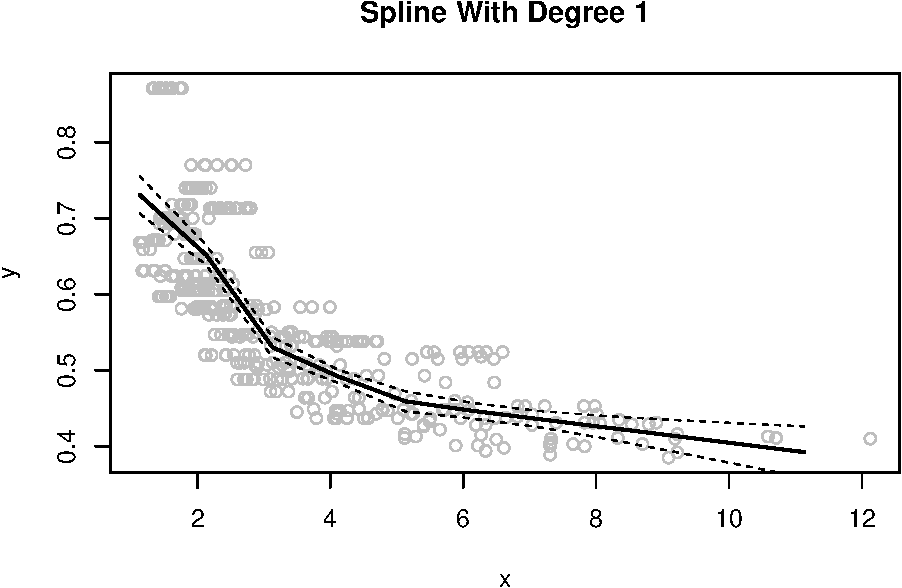
\includegraphics{hw5_files/figure-latex/unnamed-chunk-10-1.pdf}

\begin{Shaded}
\begin{Highlighting}[]
\NormalTok{MSE_var <-}\StringTok{ }\KeywordTok{c}\NormalTok{()}
\ControlFlowTok{for}\NormalTok{ (i }\ControlFlowTok{in} \DecValTok{1}\OperatorTok{:}\DecValTok{5}\NormalTok{)\{}
  \KeywordTok{print}\NormalTok{(}\KeywordTok{sd}\NormalTok{(MSE[i, ]))}
\NormalTok{  MSE_var <-}\StringTok{ }\KeywordTok{c}\NormalTok{(MSE_var, }\KeywordTok{sd}\NormalTok{(MSE[i, ]))}
\NormalTok{\}}
\end{Highlighting}
\end{Shaded}

\begin{verbatim}
## [1] 34363.53
## [1] 35195.96
## [1] 33006.79
## [1] 29038.2
## [1] 29383.97
\end{verbatim}

\begin{Shaded}
\begin{Highlighting}[]
\KeywordTok{data.frame}\NormalTok{(}\StringTok{"Complexity"}\NormalTok{ =}\StringTok{ }\DecValTok{1}\OperatorTok{:}\DecValTok{5}\NormalTok{, }\StringTok{"sd_MSE"}\NormalTok{ =}\StringTok{ }\NormalTok{MSE_var) }\OperatorTok
\StringTok{  }\KeywordTok{ggplot}\NormalTok{() }\OperatorTok{+}\StringTok{ }\KeywordTok{theme_bw}\NormalTok{() }\OperatorTok{+}
\StringTok{  }\KeywordTok{geom_line}\NormalTok{(}\KeywordTok{aes}\NormalTok{(}\DataTypeTok{x =}\NormalTok{ Complexity, }\DataTypeTok{y =}\NormalTok{ sd_MSE), }\DataTypeTok{color =} \StringTok{'maroon'}\NormalTok{, }\DataTypeTok{size =} \DecValTok{1}\NormalTok{) }\OperatorTok{+}
\StringTok{  }\KeywordTok{labs}\NormalTok{(}
    \DataTypeTok{title =} \StringTok{"MSE of the Bike Sharing Model w.r.t # of Regressors"}\NormalTok{,}
    \DataTypeTok{caption =} \StringTok{"Dataset: 2011 Washington Bike Sharing Data (Hadi Fanaee)"}
\NormalTok{  )}
\end{Highlighting}
\end{Shaded}

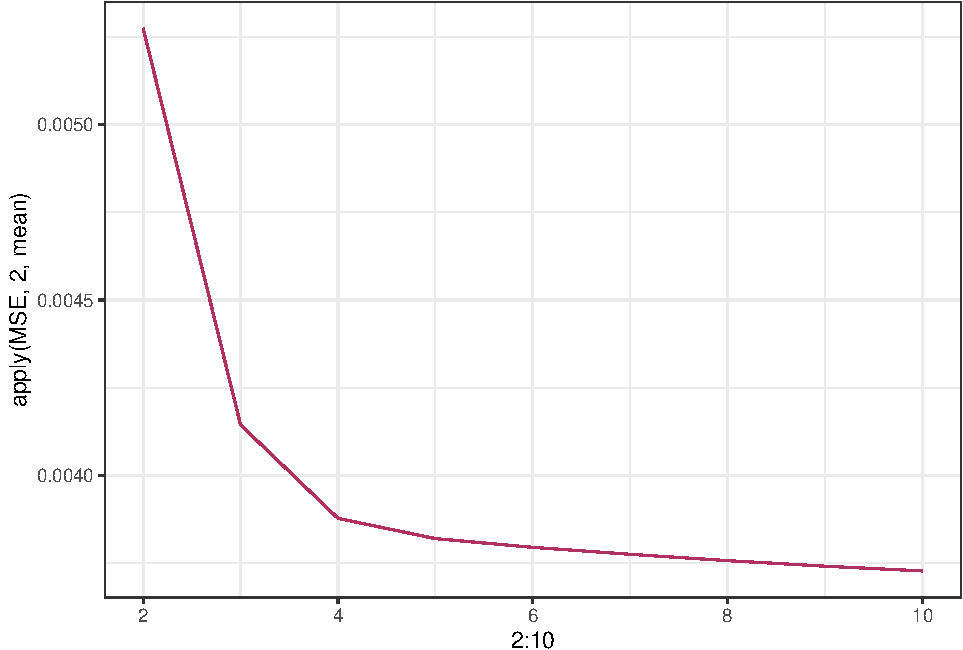
\includegraphics{hw5_files/figure-latex/unnamed-chunk-11-1.pdf}

\begin{Shaded}
\begin{Highlighting}[]
\KeywordTok{data.frame}\NormalTok{(}\StringTok{"Complexity"}\NormalTok{ =}\StringTok{ }\DecValTok{1}\OperatorTok{:}\DecValTok{5}\NormalTok{, }\StringTok{"MSE"}\NormalTok{ =}\StringTok{ }\NormalTok{MSE[}\DecValTok{1}\NormalTok{,]) }\OperatorTok
\StringTok{  }\KeywordTok{ggplot}\NormalTok{() }\OperatorTok{+}\StringTok{ }\KeywordTok{theme_bw}\NormalTok{() }\OperatorTok{+}
\StringTok{  }\KeywordTok{geom_histogram}\NormalTok{(}\KeywordTok{aes}\NormalTok{(}\DataTypeTok{x =}\NormalTok{ MSE),}\DataTypeTok{color =} \StringTok{'maroon'}\NormalTok{, }\DataTypeTok{size =} \DecValTok{1}\NormalTok{) }\OperatorTok{+}
\StringTok{  }\KeywordTok{labs}\NormalTok{(}
    \DataTypeTok{title =} \StringTok{"MSE of the Bike Sharing Model 1"}\NormalTok{,}
    \DataTypeTok{caption =} \StringTok{"Dataset: 2011 Washington Bike Sharing Data (Hadi Fanaee)"}
\NormalTok{  )}
\end{Highlighting}
\end{Shaded}

\begin{verbatim}
## `stat_bin()` using `bins = 30`. Pick better value with `binwidth`.
\end{verbatim}

\includegraphics{hw5_files/figure-latex/unnamed-chunk-12-1.pdf}

\begin{Shaded}
\begin{Highlighting}[]
\KeywordTok{data.frame}\NormalTok{(}\StringTok{"Complexity"}\NormalTok{ =}\StringTok{ }\DecValTok{1}\OperatorTok{:}\DecValTok{5}\NormalTok{, }\StringTok{"MSE"}\NormalTok{ =}\StringTok{ }\NormalTok{MSE[}\DecValTok{2}\NormalTok{,]) }\OperatorTok
\StringTok{  }\KeywordTok{ggplot}\NormalTok{() }\OperatorTok{+}\StringTok{ }\KeywordTok{theme_bw}\NormalTok{() }\OperatorTok{+}
\StringTok{  }\KeywordTok{geom_histogram}\NormalTok{(}\KeywordTok{aes}\NormalTok{(}\DataTypeTok{x =}\NormalTok{ MSE),}\DataTypeTok{color =} \StringTok{'maroon'}\NormalTok{, }\DataTypeTok{size =} \DecValTok{1}\NormalTok{) }\OperatorTok{+}
\StringTok{  }\KeywordTok{labs}\NormalTok{(}
    \DataTypeTok{title =} \StringTok{"MSE of the Bike Sharing Model 2"}\NormalTok{,}
    \DataTypeTok{caption =} \StringTok{"Dataset: 2011 Washington Bike Sharing Data (Hadi Fanaee)"}
\NormalTok{  )}
\end{Highlighting}
\end{Shaded}

\begin{verbatim}
## `stat_bin()` using `bins = 30`. Pick better value with `binwidth`.
\end{verbatim}

\includegraphics{hw5_files/figure-latex/unnamed-chunk-12-2.pdf}

\begin{Shaded}
\begin{Highlighting}[]
\KeywordTok{data.frame}\NormalTok{(}\StringTok{"Complexity"}\NormalTok{ =}\StringTok{ }\DecValTok{1}\OperatorTok{:}\DecValTok{5}\NormalTok{, }\StringTok{"MSE"}\NormalTok{ =}\StringTok{ }\NormalTok{MSE[}\DecValTok{3}\NormalTok{,]) }\OperatorTok
\StringTok{  }\KeywordTok{ggplot}\NormalTok{() }\OperatorTok{+}\StringTok{ }\KeywordTok{theme_bw}\NormalTok{() }\OperatorTok{+}
\StringTok{  }\KeywordTok{geom_histogram}\NormalTok{(}\KeywordTok{aes}\NormalTok{(}\DataTypeTok{x =}\NormalTok{ MSE),}\DataTypeTok{color =} \StringTok{'maroon'}\NormalTok{, }\DataTypeTok{size =} \DecValTok{1}\NormalTok{) }\OperatorTok{+}
\StringTok{  }\KeywordTok{labs}\NormalTok{(}
    \DataTypeTok{title =} \StringTok{"MSE of the Bike Sharing Model 3"}\NormalTok{,}
    \DataTypeTok{caption =} \StringTok{"Dataset: 2011 Washington Bike Sharing Data (Hadi Fanaee)"}
\NormalTok{  )}
\end{Highlighting}
\end{Shaded}

\begin{verbatim}
## `stat_bin()` using `bins = 30`. Pick better value with `binwidth`.
\end{verbatim}

\includegraphics{hw5_files/figure-latex/unnamed-chunk-12-3.pdf}

\begin{Shaded}
\begin{Highlighting}[]
\KeywordTok{data.frame}\NormalTok{(}\StringTok{"Complexity"}\NormalTok{ =}\StringTok{ }\DecValTok{1}\OperatorTok{:}\DecValTok{5}\NormalTok{, }\StringTok{"MSE"}\NormalTok{ =}\StringTok{ }\NormalTok{MSE[}\DecValTok{4}\NormalTok{,]) }\OperatorTok
\StringTok{  }\KeywordTok{ggplot}\NormalTok{() }\OperatorTok{+}\StringTok{ }\KeywordTok{theme_bw}\NormalTok{() }\OperatorTok{+}
\StringTok{  }\KeywordTok{geom_histogram}\NormalTok{(}\KeywordTok{aes}\NormalTok{(}\DataTypeTok{x =}\NormalTok{ MSE),}\DataTypeTok{color =} \StringTok{'maroon'}\NormalTok{, }\DataTypeTok{size =} \DecValTok{1}\NormalTok{) }\OperatorTok{+}
\StringTok{  }\KeywordTok{labs}\NormalTok{(}
    \DataTypeTok{title =} \StringTok{"MSE of the Bike Sharing Model 4"}\NormalTok{,}
    \DataTypeTok{caption =} \StringTok{"Dataset: 2011 Washington Bike Sharing Data (Hadi Fanaee)"}
\NormalTok{  )}
\end{Highlighting}
\end{Shaded}

\begin{verbatim}
## `stat_bin()` using `bins = 30`. Pick better value with `binwidth`.
\end{verbatim}

\includegraphics{hw5_files/figure-latex/unnamed-chunk-12-4.pdf}

\begin{Shaded}
\begin{Highlighting}[]
\KeywordTok{data.frame}\NormalTok{(}\StringTok{"Complexity"}\NormalTok{ =}\StringTok{ }\DecValTok{1}\OperatorTok{:}\DecValTok{5}\NormalTok{, }\StringTok{"MSE"}\NormalTok{ =}\StringTok{ }\NormalTok{MSE[}\DecValTok{5}\NormalTok{,]) }\OperatorTok
\StringTok{  }\KeywordTok{ggplot}\NormalTok{() }\OperatorTok{+}\StringTok{ }\KeywordTok{theme_bw}\NormalTok{() }\OperatorTok{+}
\StringTok{  }\KeywordTok{geom_histogram}\NormalTok{(}\KeywordTok{aes}\NormalTok{(}\DataTypeTok{x =}\NormalTok{ MSE),}\DataTypeTok{color =} \StringTok{'maroon'}\NormalTok{, }\DataTypeTok{size =} \DecValTok{1}\NormalTok{) }\OperatorTok{+}
\StringTok{  }\KeywordTok{labs}\NormalTok{(}
    \DataTypeTok{title =} \StringTok{"MSE of the Bike Sharing Model 5"}\NormalTok{,}
    \DataTypeTok{caption =} \StringTok{"Dataset: 2011 Washington Bike Sharing Data (Hadi Fanaee)"}
\NormalTok{  )}
\end{Highlighting}
\end{Shaded}

\begin{verbatim}
## `stat_bin()` using `bins = 30`. Pick better value with `binwidth`.
\end{verbatim}

\includegraphics{hw5_files/figure-latex/unnamed-chunk-12-5.pdf}


\end{document}
